% f2015gdw_q18_solid.tex — 2015 年高考数学·广东卷·文科 第 18 题（四棱锥 P-ABCD 立体图）
%
% 【来源】`.work/phase3-b16/source/2015广东文.pdf`
%   （SHA-256 0c27f1a08f837014066c636a3190b8fa7ad7e5a4494f204e60412293aea17e09），
%   第 2 页（合订本页 950）第 1 栏；内容对象 20。逐路径实测见
%   `.work/phase3-b16/figure-inventory.md` Q18 节。
%
% 【坐标口径】清单坐标为「真页 pt、原点左上、y 向下」。本图取
%   X0 = 202.0221（顶点 A 的 x），Y0 = 274.11714（顶点 A 的 y_top），
%   本地坐标  (x, y) = (x_page − X0, Y0 − y_top)，
%   即本地原点 = 顶点 A，x 向右、y 向上，1 单位 = 1 TeX pt。
%   换算示例：A (202.0221,274.1171) → (0,0)；B (365.2908,274.1171) → (163.2687,0)；
%   C (389.7813,233.3000) → (187.7592,40.8171)；D (226.5127,233.3000) → (24.4906,40.8171)；
%   P (308.1470,161.3053) → (106.1249,112.8119)。
%
% 【线宽/虚线】全部棱 line width = 0.3985pt（源先写 0.59776 w 随即被 0.3985 w 覆盖）；
%   DC 短段 dash pattern = on 2.98883pt off 2.98883pt，dash phase = 0pt；
%   无填充、无 c 算子（全为 m/l 直线）。
%
% 【照源复刻的存疑项】
%   FI-S1：DC 自 D 起为虚线，虚线终点 x=240.1184（∩ PA 计算值 x≈240.42，
%          差 0.30pt）；虚线路径方向照源为「交点 → D」，相位 0 起于交点。
%   FI-S2：源未画棱 PB，照录不补。
%   FI-S3：源每条棱路径起点有零长度重复 moveto（共 8 处），按规范不复刻。
%   FI-S9：Q18(1) 的「∥」在正文行内（y_top 89.20–98.25），不属于图形区，
%          不在本图内绘制。
%
% 【自验结果】见文件末尾。
%
% 元素计数：8 条棱（PA / PC / PD / DA / AB / BC / DC 实线 + DC 虚线）、5 个标签。
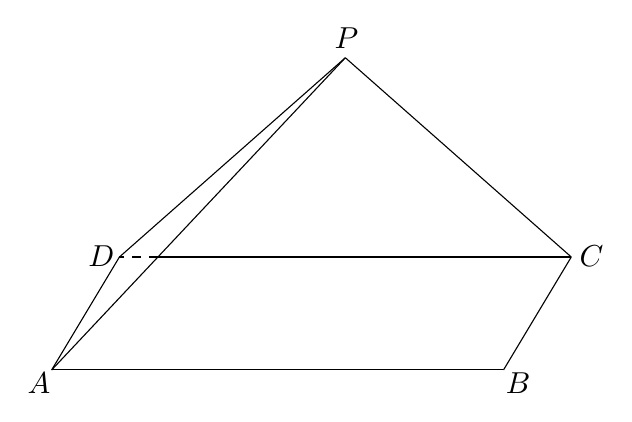
\begin{tikzpicture}[x=1pt, y=1pt,
    every node/.style={inner sep=0pt, font=\fontsize{10.5pt}{12.6pt}\selectfont}]

  % ---- 顶点（本地坐标） ----
  % A (0,0)  B (163.2687,0)  C (187.7592,40.8171)  D (24.4906,40.8171)  P (106.1249,112.8119)

  % ---- P–A（源 path 11：m A(202.0221,274.1171) l P(308.1470,161.3053)，本图反向） ----
  \draw[line width=0.3985pt] (106.1249,112.8119) -- (0.0000,0.0000);

  % ---- P–C（源 m (308.1470,161.3053) l (389.7813,233.3000)） ----
  \draw[line width=0.3985pt] (106.1249,112.8119) -- (187.7592,40.8171);

  % ---- P–D（源 path 3：m D(226.5127,233.3000) l P(308.1470,161.3053)，本图反向） ----
  \draw[line width=0.3985pt] (106.1249,112.8119) -- (24.4906,40.8171);

  % ---- D–A（源 path 7：m A(202.0221,274.1171) l D(226.5127,233.3000)，本图反向） ----
  \draw[line width=0.3985pt] (24.4906,40.8171) -- (0.0000,0.0000);

  % ---- A–B（源 path 9：m B(365.2908,274.1171) l A(202.0221,274.1171)，本图反向） ----
  \draw[line width=0.3985pt] (0.0000,0.0000) -- (163.2687,0.0000);

  % ---- B–C（源 m (365.2908,274.1171) l (389.7813,233.3000)） ----
  \draw[line width=0.3985pt] (163.2687,0.0000) -- (187.7592,40.8171);

  % ---- D–C 实线段（源 m (389.7813,233.3000) l (240.1184,233.3000)） ----
  \draw[line width=0.3985pt] (187.7592,40.8171) -- (38.0963,40.8171);

  % ---- D–C 虚线段（源 m (240.1184,233.3000) l (226.5127,233.3000)，方向照源） ----
  \draw[line width=0.3985pt, dash pattern=on 2.98883pt off 2.98883pt, dash phase=0pt]
    (38.0963,40.8171) -- (24.4906,40.8171);

  % ---- 标签：源文本 Tm 原点（基线左端），CMMI10 10.5pt ----
  \node[anchor=base west] at (102.0249,116.1981) {$P$};  % 源 (304.0470,157.9190)
  \node[anchor=base west] at (13.0239,37.2291)   {$D$};  % 源 (215.0460,236.8880)
  \node[anchor=base west] at (190.6049,37.2291)  {$C$};  % 源 (392.6270,236.8880)
  \node[anchor=base west] at (-8.8691,-8.5189)   {$A$};  % 源 (193.1530,282.6360)
  \node[anchor=base west] at (163.9539,-8.5189)  {$B$};  % 源 (365.9760,282.6360)

\end{tikzpicture}
%
% 【自验结果】
%   探针：latexmk -pdfxe，0 error / 0 Overfull / 0 Underfull / 0 Missing character；
%         页面 210.45 × 131.40 pt（standalone border=0）。
%   tex 反算：8 条棱 + 5 个标签全部匹配，最大残差 0.000057 pt（阈值 0.05）。
%   600dpi 墨迹：整体墨迹包围盒最大边差 0.285 pt；几何包围盒 0.064 pt；
%         标签中心最大 0.255 pt（C）。（尺度归一，已扣除 0.996277 的
%         TeX pt / PDF bp 均匀因子）
%         按页面 bp 直接比较（物理）最大 0.695 pt，来自该 0.37% 均匀缩放。
%   灵敏度：顶点 C x +0.15pt → tex 检查器报 0.1500、600dpi 几何包围盒报 0.1204。能报出。
